% Class
\documentclass[letterpaper, 12pt]{article}

% Language
\usepackage[spanish]{babel}

% Margin
\usepackage[margin=1in]{geometry}

% TOC Links
\usepackage{hyperref}

% Fonts
\usepackage{fontspec}
\setmainfont{Liberation Sans}
\DeclareSymbolFont{letters}{OML}{ztmcm}{m}{it} % Math Fonts

% Images
\usepackage{graphicx}
\graphicspath{{Imagenes/}} % Image directory
\usepackage{pdfpages} % Importar PDF

% Headings
\usepackage{fancyhdr}
\pagestyle{fancyplain}
\lhead{\textbf{\leftmark\space - EDO}}
\chead{}
\rhead{\textbf{Pág. \thepage\space de 14}}
\lfoot{}
\cfoot{}
\rfoot{}
\fancypagestyle{first}{
  \fancyhf[L]{}
  \fancyhf[R]{\textbf{Proyecto Final}}
  \fancyfoot{}
}

% Document Data
\title{\textbf{Solución Numérica de\\Ecuaciones Diferenciales Ordinarias}}
\author{Faustino Aguilar\footnote{Ingenieria Informatica, CRUV FIEC}\\2-732-727 \and Profesora\footnote{Análisis Numérico}\\Olga Batista}
\date{\today}

\begin{document}
  \maketitle
  \thispagestyle{first}
  \newpage
  \tableofcontents
  \thispagestyle{first}
  \newpage
  \begin{section}*{Introducción}
    \thispagestyle{first}
    \addcontentsline{toc}{section}{Introducción}
    Una ecuación diferencial ordinaria (comúnmente abreviada  \textbf{EDO}) es la ecuación diferencial que relaciona una función desconocida de una variable independiente con sus derivadas. Es decir, una sola variable independiente (a diferencia de las ecuaciones diferenciales parciales que involucran derivadas parciales de varias variables), y una o más de sus derivadas respecto de tal variable.

    Pocas ecuaciones diferenciales tienen una solución analítica sencilla, la mayor parte de las veces es necesario realizar aproximaciones, estudiar el comportamiento del sistema bajo ciertas condiciones. Así, en un sistema tan simple como un péndulo, la amplitud de la oscilación ha de ser pequeña y el rozamiento ha de ser despreciable, para obtener una solución sencilla que describa aproximadamente su movimiento periódico.

    Para la aproximación de EDO en este documento desarrollaremos:

    \begin{enumerate}
      \item Método de Euler
      \item Fórmula de Heun
      \item Método de Runge Kutta
    \end{enumerate}

    El código fuente del programa se ecuentra en un archivo adjunto a este documento.
  \end{section}
  \newpage
  \begin{section}{Método de Euler}
    \begin{subsection}{Marco Teórico}
      \begin{subsubsection}{Descripcion del problema}
        Considerando la EDO $\frac{dy}{dx} = (x -y)$ con $y(0)=-2$, encuentre una aproximación a $y(1)$.
      \end{subsubsection}
      \begin{subsubsection}{Descripcion del algoritmo}
        El método de Euler es un procedimiento de integración numérica para resolver ecuaciones diferenciales ordinarias a partir de un valor inicial dado. El método de Euler es el más simple de los métodos numéricos para resolver un problema de valor inicial.

        Este método consiste en calcular de forma iterativa:
        \[h = (b - a)/2\]
        \[y_i = y_{i-1} + hf(x_{i-1},y_{i-1})\]
        \[x_i = x_{i-1} + h\]
      \end{subsubsection}
    \end{subsection}
    \begin{subsection}{Descripción de variables}
      \begin{table}[h]
        \centering
        \begin{tabular}{|c c c|}
          \hline
          Nombre & Tipo & Utilidad\\
          \hline\hline
          n & entero & Cantidad de intervalos \\
          i & entero & Contador \\
          h & real & Delta x \\
          a & real & Valor inicial \\
          b & real & Valor a encontrar \\
          x & real & Valor para almacenar xi \\
          y & real & Valor para almacenar yi\\
          f & real & Funcion para calcular f(x,y) \\
          \hline
        \end{tabular}
        \caption{Método de Euler: Variables utilizadas}
      \end{table}
    \end{subsection}
    \newpage
    \begin{subsection}{Diagrama de Flujo}
      \begin{figure}[h]
        \centering
        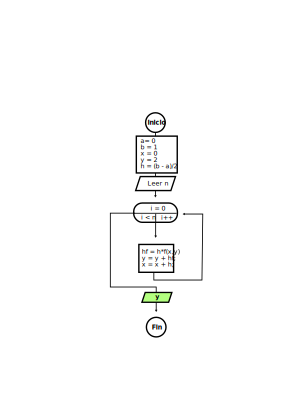
\includepdf[pages={1}]{Imagenes/euler.pdf}
        \caption{Diagrama de flujo del Método de Euler}
      \end{figure}
    \end{subsection}
    \newpage
    \begin{subsection}{Resultados}
      La ecuacion $y' = x -y$ resuelta analíticamente tiene como solución $y = 3e^{-x} +x -1$, si la evaluamos en $y(1)=1,10364$, entonces el error relativo es:
      \[Error = \frac{1,10364 - 1.1122}{1,10364} = 0.1092\]
      \begin{figure}[h]
        \centering
        \includegraphics[scale=1.0]{Euler.png}
        \caption{Resultados del Método de Euler}
      \end{figure}
    \end{subsection}
  \end{section}
  \newpage
  \begin{section}{Fórmula de Heun}
    \begin{subsection}{Marco Teórico}
      \begin{subsubsection}{Descripcion del problema}
        Considerando la EDO $\frac{dy}{dx} = (x -y)$ con $y(0)=-2$, encuentre una aproximación a $y(1)$.
      \end{subsubsection}
      \begin{subsubsection}{Descripcion del algoritmo}
        La mejora del método de Heun consiste en la aproximación a la pendiente mediante la aplicación de dos derivadas del intervalo, una en el punto inicial y otra en punto final. La aproximación mejorada de la pendiente será el promedio de las dos derivadas.

        Este método consiste en calcular de forma iterativa:
        \[h = (b - a)/2\]
        \[k_1 = f(x_{i-1}, y_{i-1})\]
        \[y^0 = y_{i-1} + hk_1\]
        \[x_i = x_{i-1} + h\]
        \[k_1 = f(x_i, y^0)\]
        \[y_i = y_{i-1} + h(k_1 + k_2)/2\]
      \end{subsubsection}
    \end{subsection}
    \begin{subsection}{Descripción de variables}
      \begin{table}[h]
        \centering
        \begin{tabular}{|c c c|}
          \hline
          Nombre & Tipo & Utilidad\\
          \hline\hline
          n & entero & Cantidad de intervalos \\
          i & entero & Contador \\
          h & real & Delta x \\
          a & real & Valor inicial \\
          b & real & Valor a encontrar \\
          x & real & Valor para almacenar xi \\
          yi & real & Valor para almacenar yi\\
          k1 & real & Valor para almacenar k1 = f(x,yi)\\
          y0 & real & Valor para almacenar y0 = yi + h*k1\\
          k2 & real & Valor para almacenar k2 = f(xi,y0)\\
          f & real & Funcion para calcular f(x,y) \\
          \hline
        \end{tabular}
        \caption{Fórmula de Heun: Variables utilizadas}
      \end{table}
    \end{subsection}
    \newpage
    \begin{subsection}{Diagrama de Flujo}
      \begin{figure}[h]
        \centering
        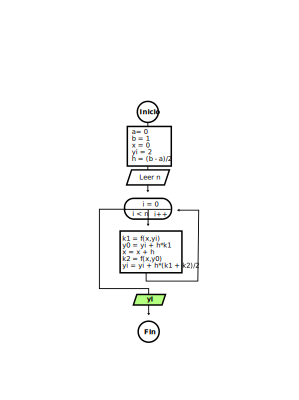
\includepdf[pages={1}]{Imagenes/heun.pdf}
        \caption{Diagrama de flujo del Método de Heun}
      \end{figure}
    \end{subsection}
    \newpage
    \begin{subsection}{Resultados}
      La ecuacion $y' = x -y$ resuelta analíticamente tiene como solución $y = 3e^{-x} +x -1$, si la evaluamos en $y(1)=1,10364$, entonces el error relativo es:
      \[Error = \frac{1,10364 - 1.1122}{1,10364} = 0.0077\]
      \begin{figure}[h]
        \centering
        \includegraphics[scale=1.0]{Heun.png}
        \caption{Resultados del Método de Heun}
      \end{figure}
    \end{subsection}
  \end{section}
  \newpage
  \begin{section}{Método de Runge Kutta}
    \begin{subsection}{Marco Teórico}
      \begin{subsubsection}{Descripcion del problema}
        Considerando la EDO $\frac{dy}{dx} = (x -y)$ con $y(0)=-2$, encuentre una aproximación a $y(1)$.
      \end{subsubsection}
      \begin{subsubsection}{Descripcion del algoritmo}
        Los métodos de Runge-Kutta (RK) son un conjunto de métodos iterativos para la aproximación de soluciones de ecuaciones diferenciales ordinarias con valor inicial.

        Este método consiste en calcular de forma iterativa:
        \[h = (b - a)/2\]
        \[k_1 = f(x_{i-1}, y_{i-1})\]
        \[k_2 = f(x_{i-1} + h/2, y_{i-1} + k_1h/2)\]
        \[k_3 = f(x_{i-1} + h/2, y_{i-1} + k_2h/2)\]
        \[k_4 = f(x_{i-1} + h, y_{i-1} + k_3h)\]
        \[x_i = x_{i-1} + h\]
        \[y_i = y_{i-1} + h(k_1 + 2k_2 + 2k_3 + k_4)/6\]
      \end{subsubsection}
    \end{subsection}
    \begin{subsection}{Descripción de variables}
      \begin{table}[h]
        \centering
        \begin{tabular}{|c c c|}
          \hline
          Nombre & Tipo & Utilidad\\
          \hline\hline
          n & entero & Cantidad de intervalos \\
          i & entero & Contador \\
          h & real & Delta x \\
          a & real & Valor inicial \\
          b & real & Valor a encontrar \\
          x & real & Valor para almacenar xi \\
          y & real & Valor para almacenar yi\\
          k1 & real & Valor para almacenar f(x,y)\\
          k2 & real & Valor para almacenar f(x + h/2, y + k1*h/2)\\
          k2 & real & Valor para almacenar f(x + h/2, y + k2*h/2)\\
          k2 & real & Valor para almacenar f(x + h, y + k3*h)\\
          f & real & Funcion para calcular f(x,y) \\
          \hline
        \end{tabular}
        \caption{Método de Runge Kutta: Variables utilizadas}
      \end{table}
    \end{subsection}
    \newpage
    \begin{subsection}{Diagrama de Flujo}
      \begin{figure}[h]
        \centering
        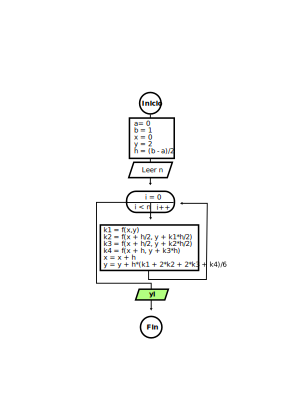
\includepdf[pages={1}]{Imagenes/runge.pdf}
        \caption{Diagrama de flujo del Método de Runge Kutta}
      \end{figure}
    \end{subsection}
    \newpage
    \begin{subsection}{Resultados}
      La ecuacion $y' = x -y$ resuelta analíticamente tiene como solución $y = 3e^{-x} +x -1$, si la evaluamos en $y(1)=1,10364$, entonces el error relativo es:
      \[Error = \frac{1,10364 - 1.10366}{1,10364} = 0.00001\]
      \begin{figure}[h]
        \centering
        \includegraphics[scale=1.0]{Runge.png}
        \caption{Resultados del Método de Runge-Kutta}
      \end{figure}
    \end{subsection}
  \end{section}
  \newpage
  \begin{section}{Conclusiones}
    En este presente trabajo tengo puedo concluir que:
    \begin{description}
      \item[Método de Euler:] este método al ser analizado ha resultado en tener un gran margen de error por lo que requiere una mayor cantidad de intervalos para tener más exactitud. su ventaja es que es un método bastante sencillo.
      \item[Fórmula de Heun:] este es una mejora al método de Euler. Se ve claramente como se hace una pequeña modificación en el calculo, calculando el promedio de calculos intermedios para mejorar el margen de error.
      \item[Método de Runge Kutta:] el método más exacto de todos, permitiendo un margen de error de micro decimales, algo bastante bueno cuando se busca exactitud, pero el un método que requiere mayor capacidad de calculo.

      En mi experiencia me ha gustado más el Método de Runge-Kuta por su forma de implementar los calculos de las iteraciones.
    \end{description}
  \end{section}
  \newpage
  \nocite{*}
  \begin{bibliography}{bibliografia}
    \bibliographystyle{apalike}
    \addcontentsline{toc}{section}{Bibliografía}
  \end{bibliography}
\end{document}
